\usepackage{tikz}
\usetikzlibrary{positioning, shapes.geometric, arrows.meta, calc, fit, backgrounds}

% Custom Colors for Publication
\definecolor{headcolor}{RGB}{200, 230, 201} % Light Green
\definecolor{faiiacolor}{RGB}{255, 243, 224} % Light Orange
\definecolor{grayblock}{RGB}{245, 245, 245} % Neutral Gray
\definecolor{linecolor}{RGB}{100, 100, 100} % Dark Gray for lines

\tikzset{
    base/.style={rectangle, draw, thick, rounded corners=2pt, minimum height=0.8cm, text centered, font=\small, inner sep=4pt},
    input/.style={base, fill=grayblock, minimum width=1.5cm},
    process/.style={base, fill=white, minimum width=2.5cm},
    faiia/.style={base, fill=faiiacolor, minimum width=4cm, solid, draw=orange!70},
    aux/.style={base, fill=headcolor!40, minimum width=2.5cm, dashed},
    arrow/.style={-{Stealth[scale=1.2]}, thick, draw=linecolor},
    label_text/.style={font=\scriptsize\itshape, text=linecolor}
}

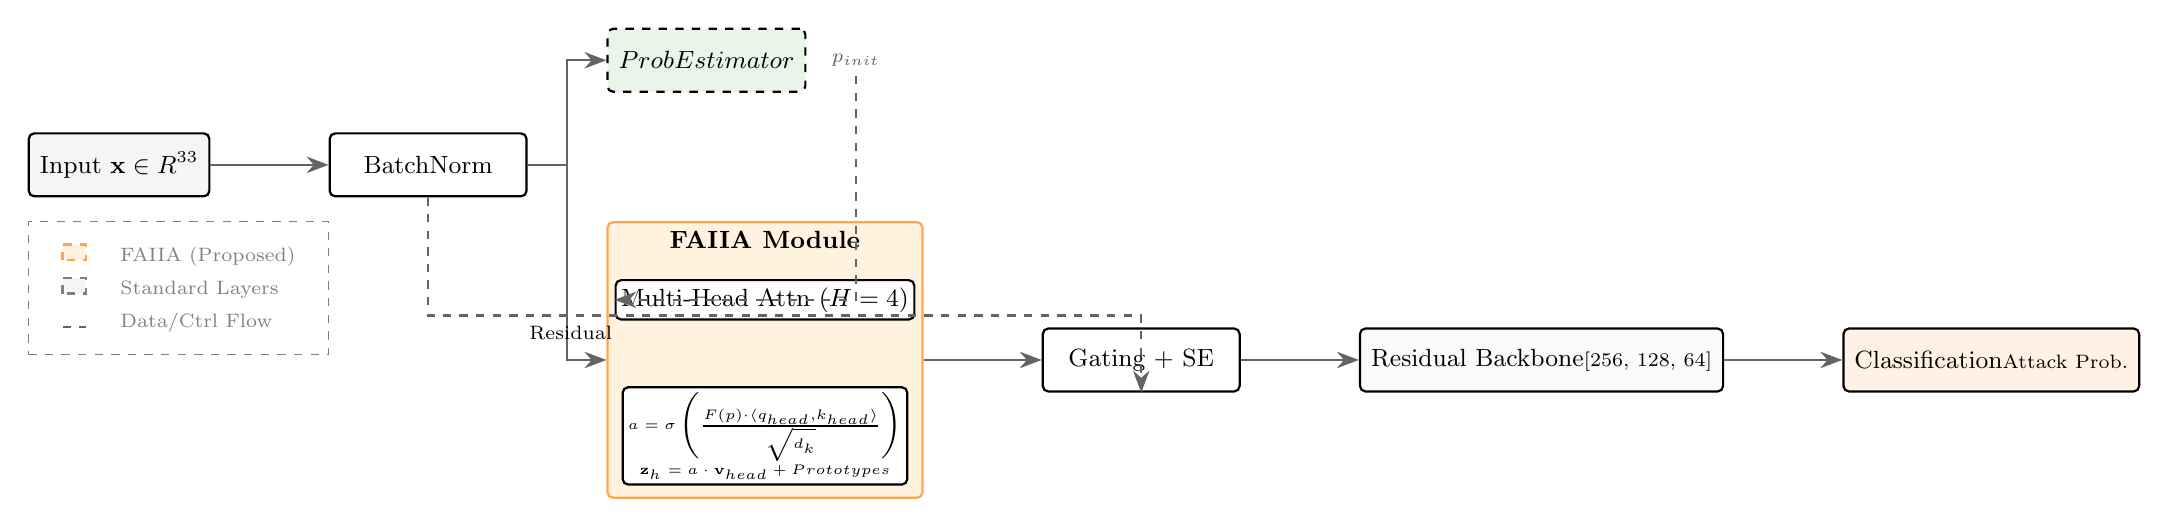
\begin{tikzpicture}[node distance=1.2cm and 1.5cm, >=stealth]

    % --- Column 1: Input ---
    \node [input] (in) {Input $\mathbf{x} \in \mathbb{R}^{33}$};
    \node [process, right=of in] (bn) {BatchNorm};
    \draw [arrow] (in) -- (bn);

    % --- Column 2: Dual Path ---
    \node [aux, above right=0.5cm and 1cm of bn] (prob) {$\text{Prob Estimator}$};
    \node [faiia, below right=0.3cm and 1cm of bn, minimum height=3.5cm] (faiia_box) {};
    
    % Connections from BN
    \draw [arrow] (bn.east) -- ++(0.5,0) |- (prob.west);
    \draw [arrow] (bn.east) -- ++(0.5,0) |- (faiia_box.west);

    % Internal FAIIA Structure
    \node [font=\bfseries\small, anchor=north] at (faiia_box.north) {FAIIA Module};
    
    \node [base, fill=white, inner sep=2pt, minimum height=0.5cm] (heads) at ([yshift=-1cm]faiia_box.north) {Multi-Head Attn ($H=4$)};
    \node [base, fill=white, inner sep=2pt, minimum height=1cm, font=\tiny, align=center] (score) at ([yshift=0.8cm]faiia_box.south) {
        $a = \sigma\left(\frac{F(p) \cdot \langle q_{head}, k_{head} \rangle}{\sqrt{d_k}}\right)$ \\
        $\mathbf{z}_{h} = a \cdot \mathbf{v}_{head} + \text{Prototypes}$
    };
    
    % Focal Link
    \node [label_text, right=0.2cm of prob] (p_out) {$p_{init}$};
    \draw [arrow, dashed] (p_out) |- (heads.west);

    % --- Column 3: Feature Refinement ---
    \node [process, right=of faiia_box] (gate) {Gating + SE};
    \draw [arrow] (faiia_box) -- (gate);
    
    % Residual Link from BN to Gate
    \draw [arrow, dashed] (bn.south) -- ++(0,-1.5) -| (gate.south) node[pos=0.1, below] {\scriptsize Residual};

    % --- Column 4: Deep FE ---
    \node [process, right=of gate, fill=grayblock!50] (dfe) {Residual Backbone \\ \scriptsize [256, 128, 64]};
    \draw [arrow] (gate) -- (dfe);

    % --- Column 5: Output ---
    \node [input, right=of dfe, fill=orange!10] (out) {Classification \\ \scriptsize Attack Prob.};
    \draw [arrow] (dfe) -- (out);

    % Legend
    \node [draw, dashed, gray, rounded corners=0, inner sep=6pt, anchor=south west] at ([yshift=-2cm]in.south west) (legend) {
        \begin{tabular}{ll}
            \tikz\draw[thick, orange!70, fill=faiiacolor] (0,0) rectangle (0.3,0.2); & \scriptsize FAIIA (Proposed) \\
            \tikz\draw[thick, gray, fill=grayblock] (0,0) rectangle (0.3,0.2); & \scriptsize Standard Layers \\
            \tikz\draw[thick, dashed, draw=linecolor] (0,0) -- (0.3,0); & \scriptsize Data/Ctrl Flow
        \end{tabular}
    };

\end{tikzpicture}
